% This file was created with tikzplotlib v0.10.1.
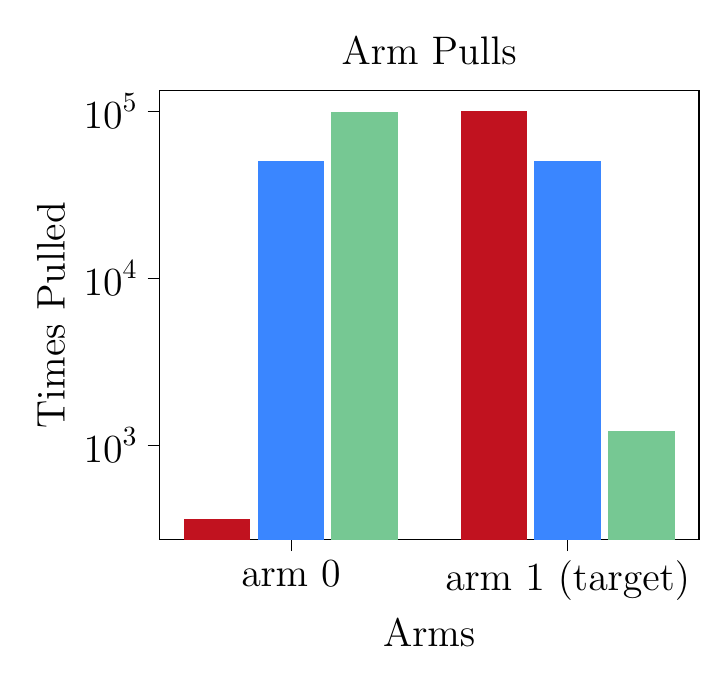
\begin{tikzpicture}[
every node/.append style={font=\Large}
]

\definecolor{darkgray176}{RGB}{176,176,176}
\definecolor{darkseagreen118200147}{RGB}{118,200,147}
\definecolor{dodgerblue58134255}{RGB}{58,134,255}
\definecolor{firebrick1931831}{RGB}{193,18,31}
\definecolor{lightgray204}{RGB}{204,204,204}

\begin{axis}[
legend cell align={left},
legend style={fill opacity=0.8, draw opacity=1, text opacity=1, draw=lightgray204},
log basis y={10},
tick align=outside,
tick pos=left,
title={Arm Pulls},
x grid style={darkgray176},
xlabel={Arms},
xmin=-0.475333333333333, xmax=1.47533333333333,
xtick style={color=black},
xtick={0,1},
xticklabels={arm 0,arm 1 (target)},
y grid style={darkgray176},
ylabel={Times Pulled},
ymin=273.669523207196, ymax=131942.591987717,
ymode=log,
ytick style={color=black},
ytick={10,100,1000,10000,100000,1000000,10000000},
yticklabels={
  \(\displaystyle {10^{1}}\),
  \(\displaystyle {10^{2}}\),
  \(\displaystyle {10^{3}}\),
  \(\displaystyle {10^{4}}\),
  \(\displaystyle {10^{5}}\),
  \(\displaystyle {10^{6}}\),
  \(\displaystyle {10^{7}}\)
}
]
\draw[draw=none,fill=firebrick1931831] (axis cs:-0.386666666666667,0) rectangle (axis cs:-0.146666666666667,362.4);
\draw[draw=none,fill=firebrick1931831] (axis cs:0.613333333333333,0) rectangle (axis cs:0.853333333333333,99637.6);
\draw[draw=none,fill=dodgerblue58134255] (axis cs:-0.12,0) rectangle (axis cs:0.12,49986);
\draw[draw=none,fill=dodgerblue58134255] (axis cs:0.88,0) rectangle (axis cs:1.12,50014);
\draw[draw=none,fill=darkseagreen118200147] (axis cs:0.146666666666667,0) rectangle (axis cs:0.386666666666667,98778.3);
\draw[draw=none,fill=darkseagreen118200147] (axis cs:1.14666666666667,0) rectangle (axis cs:1.38666666666667,1221.7);
\end{axis}

\end{tikzpicture}
